%%%%%%%%%%%%%%%%%%%%%% Generalities %%%%%%%%%%%%%%%%%%5
\documentclass[11pt,fleqn]{amsart}
%\usepackage[paper=a4paper]
 %{geometry}

\pagestyle{plain}
\pagenumbering{arabic}
%%%%%%%%%%%%%%%%%%%%%%%%%%%%%%%%
\usepackage[small]{titlesec}
\usepackage{hyperref}
\usepackage{amsthm,thmtools}
%\usepackage{showlabels}
\linespread{1.05}
%\setlength{\parskip}{1.2ex}

\usepackage[utf8]{inputenc}
\usepackage[english]{babel}
\usepackage{enumerate}
\usepackage[osf,noBBpl]{mathpazo}
\usepackage[alphabetic,initials]{amsrefs}
\usepackage{amsfonts,amssymb,amsmath}
\usepackage{mathtools}
\usepackage{graphicx}
\usepackage[poly,arrow,curve,matrix]{xy}
%\usepackage{wrapfig}
%\usepackage{xcolor}
\usepackage{helvet}
\usepackage{stmaryrd}
\usepackage{tikz}
%\usepackage{mathdots}
%\usepackage[normalem]{ulem}

\renewcommand\thesection{\arabic{section}}
\titleformat{\section}
 {\normalfont\bfseries\large}
 {\thesection. \space}{0em}{}

\renewcommand\thesubsection{\arabic{subsection}}
\titleformat{\subsection}
 {\normalfont\bfseries}
 {\thesection.\thesubsection \space}{0em}{}

\renewcommand\proofname{Proof}

\makeatletter
\renewenvironment{proof}[1][\textit{\proofname}]{\par
 \pushQED{\qed}%
 \normalfont \topsep.75\paraskip\relax
 \trivlist
 \item[\hskip\labelsep
 \itshape
 #1\@addpunct{.}]\ignorespaces
}{%
 \popQED\endtrivlist\@endpefalse
}
\makeatother
%%%%%%%%%%%%%%%%%%%%%%%%%%% Theorems et al%%%%%%%%%%%%%%%%%%%%%%%%%%
\declaretheoremstyle[
%headformat=swapnumber, 
bodyfont=\itshape,]{mystyle}
\declaretheorem[name=Lemma, style=mystyle, numberwithin=section]{Lemma}
\declaretheorem[name=Proposition, style=mystyle, sibling=Lemma]{Proposition}
\declaretheorem[name=Theorem, style=mystyle, sibling=Lemma]{Theorem}
\declaretheorem[name=Corollary, style=mystyle, sibling=Lemma]{Corollary}
\declaretheorem[name=Definition, style=mystyle, sibling=Lemma]{Definition}
\declaretheorem[name=Example, style=mystyle, sibling=Lemma]{Example}
\declaretheorem[name=Remark, style=mystyle, sibling=Lemma]{Remark}

% unnumbered versions
\declaretheoremstyle[numbered=no, 
bodyfont=\itshape]{mystyle-empty}
\declaretheorem[name=Lemma, style=mystyle-empty]{Lemma*}
\declaretheorem[name=Proposition, style=mystyle-empty]{Proposition*}
\declaretheorem[name=Theorem, style=mystyle-empty]{Theorem*}
\declaretheorem[name=Corollary, style=mystyle-empty]{Corollary*}
\declaretheorem[name=Definition, style=mystyle-empty]{Definition*}
\declaretheorem[name=Example, style=mystyle-empty]{Example*}
\declaretheorem[name=Remark, style=mystyle-empty]{Remark*}

%%%%%%%%%%%%%%%%%%%%%%%%%%% Paragraphs %%%%%%%%%%%%%%%%%%%%%%%%%%%%%
\newskip\paraskip
\paraskip=0.75ex plus .2ex minus .2ex

\newcounter{para}[section]
\setcounter{para}{0}
\renewcommand\thepara{\thesection.\arabic{para}}
\def\paragraph{%
 \noindent
 \refstepcounter{para}%
 \textbf{\thepara.}\hspace{1ex}%
}

\newcommand\about[1]{%
 {\bfseries#1.}%
}

\newcommand\pref[1]{\textbf{\ref{#1}}}

\renewcommand\theHpara{\theHsection.\arabic{para}}
%%%%%%%%%%%%%%%%%%%%%%%%%%% The usual stuff%%%%%%%%%%%%%%%%%%%%%%%%%
\newcommand\NN{\mathbb N}
\newcommand\CC{\mathbb C}
\newcommand\QQ{\mathbb Q}
\newcommand\RR{\mathbb R}
\newcommand\ZZ{\mathbb Z}
\newcommand\PiI{\mathbb I}
\renewcommand\k{\Bbbk}

\newcommand\maps{\longmapsto}
\newcommand\ot{\otimes}
\renewcommand\to{\longrightarrow}
\renewcommand\phi{\varphi}
\newcommand\Pid{\mathsf{Id}}
\newcommand\im{\mathsf{im}}
\newcommand\coker{\mathsf{coker}}
%%%%%%%%%%%%%%%%%%%%%%%%% Specific notation %%%%%%%%%%%%%%%%%%%%%%%%%
%\newcommand\Pi{\mathcal I}
%\newcommand\Pi'{\mathcal J}
\newcommand\D[3]{{}^{#1} \mathfrak D_{#2}^{#3}}
\newcommand\DD[3]{{}^{#1} \mathcal D_{#2}^{#3}}
\newcommand\Z{\mathsf Z}

\newcommand\g{\mathfrak g}
\newcommand\p{\mathfrak p}
\newcommand\m{\mathfrak m}
\newcommand\gl{\mathfrak{gl}}
\newcommand\gen{\mathsf{gen}}
\newcommand\std{\mathsf{std}}
\newcommand\sh{\mathsf{sh}}
\renewcommand\SS{\mathfrak S}
\newcommand\vv{\overline{v}}

\newcommand\vectspan[1]{\left\langle #1 \right\rangle}
\newcommand\interval[1]{\llbracket #1 \rrbracket}

\DeclareMathOperator\Frac{Frac}
\DeclareMathOperator\Specm{Specm}
\DeclareMathOperator\End{End}
\DeclareMathOperator\Hom{Hom}

\DeclareMathOperator\sym{sym}
\DeclareMathOperator\asym{asym}
\DeclareMathOperator\sg{sg}
\DeclareMathOperator\ev{\mathsf{ev}}
\DeclareMathOperator\ann{ann}
\DeclareMathOperator\supp{supp}

\newcommand\Desc[1]{\mathbb D(#1)}

\newcommand\bigmodule{big GT module~}

%%%%%%%%%%%%%%%%%%%%%%%%%%%%%%%%%%%%%% TITLES %%%%%%%%%%%%%%%%%%%%%%%%%%%%%%
\title{On the structure of the Big GT-module associated to a character}
%\author{[structure.tex]}
\date{}


\begin{document}
\maketitle
%\vspace{-2cm}
The \bigmodule is the one built in \cite{RZ18}.

\section{Notation}
Fix $n \in \NN$ and let $\mu = (n, n-1, \ldots, 1)$. 
Given $a,b,k \in \NN$ we set 
$\interval{a,b} = \{i \in \NN \mid a \leq i \leq b\}$ and $\interval{b} = 
\interval{1,b}$; also set $\interval{a,b}_k = \{(k,i) \mid i \in 
\interval{a,b}\}$. If $I = \interval{a,b}$ we define $a(I) = a$ and $b(I)=b$, 
so $|I| = b(I) - a(I) + 1$. Given $\mu = (\mu_1, \ldots, \mu_n) \in \NN^n$
we write $\Sigma(\mu) = \{\interval{\mu_k}_k \mid 1 \leq k \leq n\} = \{(k,i) 
\mid k \in \interval{n}, i \in \interval{\mu_k}\}$.

\paragraph
Let $r \in \NN$ and $v \in \CC^r$. We say that $v$ is in \emph{normal form} if 
whenever $v_i - v_j \in \ZZ$ for $i > j$, then $v_{i'} - v_{j'} \in \ZZ_{\geq 
0}$ for all $i' > j'$ where $i',j' \in \interval{i,j}$. 

The symmetric group $S_r$ acts on $\CC^r$ by permuting the entries of an 
element. This is a Coxeter group with generating set given by simple 
transpositions $(i,i+1)$ for $1 \leq i \leq r-1$. For each $\sigma \in S_r$
we will denote by $\ell(\sigma)$ the length of the element $\sigma$ with 
respect to this generating set. Given $v \in \CC^r$ there is at least one 
element in its $S_r$-orbit which is in normal form. If $v$ is in normal form 
then its stabilizer $(S_r)_v$ is generated by those $(i,i+1)$ such that $v_i = 
v_{i+1}$ and hence it is a parabolic subgroup of $S_r$. Each coclass $S_r/
(S_r)_v$ has a unique representative of minimal length. We denote by $S_r^v$ 
the collection of these representatives, and we call them $v$-shuffles. A 
permutation $\sigma \in S_r$ is a $v$-shuffle if and only if for all $i < j, 
i,j \in \interval r$ such that $v_i = v_j$ we have $\sigma(i) < \sigma(j)$. 

\paragraph
\about{Partitions and compositions}
\label{partitions-compositions}
Fix $\mu \in \NN^n$ and put $\Sigma = \Sigma(\mu)$. An interval of $\Sigma$ is 
a set $\interval{a,b}_k \subset \Sigma$. A composition $\Pi$ of $\Sigma$ is a 
disjoint family of intervals of $\Sigma$, whose union is $\Sigma$. Given a 
composition $\Pi$ of $\Sigma$ and $k \in \interval n$, we denote by $\Pi_k$ the
set of all intervals $\interval{a,b}_k \in \Pi$. Given two compositions $\Pi, 
\Pi'$ of $\Sigma$, we say that $\Pi'$ refines $\Pi$ and write $\Pi' < \Pi$ if 
for each $J \in \Pi'$ there exists $I \in \Pi$ such that $J \subset I$. 

A composition of $\mu$ is an $n$-tuple $\pi = (\pi^{(1)}, \ldots, 
\pi^{(n)})$ where $\pi^{(k)}$ is a composition of $k$. To each
composition $\Pi$ of $\Sigma$ we assign a composition $\pi(\Pi)$ of $\mu$, 
setting $\pi^{(k)}_j$ to be the cardinality of the $j$-th interval in $\Pi_k$. 
This assignation is bijective, and for each composition $\pi$ of $\mu$ we 
denote by $\Pi(\pi)$ the unique composition of $\Sigma$ corresponding to 
$\pi$. We say that a composition $\epsilon$ refines $\pi$, and write 
$\epsilon < \pi$, whenever $\Pi(\epsilon) < \Pi(\pi)$. Compositions of $\mu$ 
form a finite poset with maximum $\mu$, so whenever we write $\pi < \mu$ we 
will mean that $\pi$ is a composition of $\mu$.

For each finite set $X$ we denote by $S(X)$ the set of all bijections from
$X$ to $X$. Set $S_\mu = S(\interval{\mu_1}_1) \times S(\interval{\mu_2}_{2}) 
\times \cdots \times S(\interval{\mu_n}_n)$, which is a subset of $S(\Sigma)$. 
Every element $\sigma \in S_\mu$ can be written as $\sigma_{(1)} \sigma_{(2)}
\cdots \sigma_{(n)}$ with $\sigma_{(k)} \in S(\interval{k}_k)$. Obviously
$S(\interval{\mu_k}_k)$ is isomorphic to the symmetric group in $\mu_k$ 
elements, and given a permutation $\sigma \in S_{\mu_k}$ we will denote the 
corresponding element of $S(\interval{\mu_k}_k)$ by $\sigma_{(k)}$. 

If $I \subset \Sigma$ is an interval then we see $S(I) \subset S_\mu$ in the 
obvious way. For each composition $\Pi$ of $\Sigma$ we define $S_\Pi = 
\prod_{I \in \Pi} S(I) \subset S_\mu$, and for each $\pi < \mu$ we set $S_\pi 
= S_{\Pi(\pi)}$. Since it is a product of symmetric groups, $S_\mu$ is a 
Coxeter group with generating set $\{(i,i+1)_{(k)} \mid 1 \leq i \leq \mu_k-1, 
1 \leq k \leq n\}$, and each $S_\pi$ is a parabolic subgroup of $S_\mu$. The
length of an element $\sigma \in S_\mu$ will always be taken with respect to
this set of generators.

\paragraph
\about{$\mu$-points}
\label{mu-points}
Set $\CC^\mu = \CC^{\mu_1} \times \CC^{\mu_2} \times \cdots \times 
\CC^{\mu_n}$. A point in $\CC^\mu$ is thus an $n$-tuple $(v_n, \ldots, v_1)$ 
with each $v_k$ a vector with $\mu_kk$ entries. We will refer to the $v_k$'s 
as the \emph{rows} of $v$ and denote by $v_{k,i}$ the $i$-th entry of $v_k$. 
Also given an interval $\interval{a,b}_k \subset \Sigma$ we write 
$v(\interval{a,b}_k) = (v_{k,a},\ldots, v_{k,b})$. Given $\pi < \mu$ and $\Pi 
= \Pi(\pi)$ the $\pi$-blocks of $v$ are the elements of the set $\{v(I) \mid 
I \in \Pi\}$. The group $S_\mu$ acts on $\CC^\mu$ by permuting the entries, 
i.e. $\sigma(v)_{k,i} = v_{\sigma(k,i)} = v_{k,\sigma_{(k)}(i)}$. 

We will say that $v \in \CC^\mu$ is in \emph{normal form} if each of its rows 
is in normal form. Clearly every $S_\mu$-orbit of $\CC^\mu$ contains at least 
one point in normal form, and if $v$ is in normal form then its stabilizer is 
a standard parabolic subgroup generated by the set $\{(i,i+1)_k \mid v_{k,i} = 
v_{k,i+1}\}$. The isomorphism $S_\mu \cong \prod_{k \in \interval n} 
S_{\mu_k}$ sends the stabilizer $(S_\mu)_v$ to the product $\prod_{k \in 
\interval n} (S_{\mu_k})_{v_k}$. Each coclass in $S_\mu/ (S_\mu)_v$ contains 
an element of minimal length, which is of the form $\sigma_{(1)} \sigma_{(2)} 
\cdots \sigma_{(n)}$ with $\sigma_{(k)}$ a $v_k$-shuffle. We denote the set of 
all these minimal length representatives by $S_\mu^v$ and refer to them as 
$v$-shuffles. As before, $\sigma$ is a $v$-shuffle if and only if whenever
$v_{k,i} = v_{k,j}$ and $i<j$ then $\sigma(i) < \sigma(j)$.

A $\mu$-point $v$ induces an equivalence relation in $\Sigma$ as follows:
we will say that $(k,i)$ is equivalent to $(l,j)$ if $l=k \neq n$ and $v_{k,i}
= v_{k,j}$. If $v$ is in normal form then the equivalence classes of this
relation form a composition $\Pi(v)$ of $\Sigma$. We denote by $\pi(v)$ the
corresponding composition of $\mu$.

\paragraph
We set $\Lambda = \CC[x_{k,i} \mid (k,i) \in \Sigma]$, the ring of polynomial 
functions on $\CC^\mu$, and by $K = \Frac(\Lambda)$ its fraction field. The 
action of $S_\mu$ on $\CC^\mu$ induces an action on $\Lambda$ which is given 
by $\sigma(x_{k,i}) = x_{\sigma(k,i)} = x_{k,\sigma_{(k)}(i)}$, and extends to 
the fraction field. If $\pi < \mu$ then $S_\pi$ acts on $\CC^\mu$ by 
restriction, which induces $S_\pi$ actions on $\Lambda$ and $K$. Notice that
the action of $S_\pi$ only permutes elements in the same $\pi$-block.

\paragraph
We denote by $\ZZ^\mu_0 \subset \CC^\mu$ the set of points with integral 
entries and $z_{n,i} = 0$ for all $i \in \interval{\mu_n}$. Fix $\pi < \mu$ 
and let $\Pi = \Pi(\pi)$ be the corresponding composition of $\Sigma$. We say 
that $z \in \ZZ^\mu_0$ is \emph{$\pi$-standard}, or just standard if $\pi$ is 
clear from the context, if for each $\interval{a,b}_k \in \Pi(\pi)$ we have 
$z_{k,a} \geq z_{k,a+1} \geq \cdots \geq z_{k,b}$; in other words, each 
$\pi$-block of $z$ is a weakly decreasing sequence. For each $z \in \ZZ^\mu_0$
there is exactly one element in the orbit $S_\pi z$ which is $\pi$-standard, 
and we denote it by $\std_\pi(z)$. Thus the set $\std(\pi) = \{\std_\pi(z) 
\mid \ZZ^\mu_0\}$ is a complete set of representatives of the equivalence 
classes in $\ZZ^\mu_0 /S_\pi$. 

If $z \in \std(\pi)$ then there existes a refinement $\epsilon(z) < \pi$ 
such that $S_{\epsilon(z)}$ is the stabilizer of $z$ in $S_\pi$. The 
corresponding partition is denoted by $E(z)$. 


\section{The modules}
From now on we fix $\mu = (1,2,\ldots, n)$ and $\Sigma = \Sigma(\mu)$.

Let $v \in \CC^\mu$. We build a graph with vertex set $\Sigma$, with 
an edge between $(k,i)$ and $(l,j)$ if and only if $k,l < n$, $v_{k,i} - 
v_{l,j} \in \ZZ$, and $|k-l| \leq 1$. We will say that $(k,i)$ and $(l,j)$
are $v$-related if and only if they lie in the same connected component of
$v$.

\begin{Example}
In each case we have drawn an edge between related entries in the 
corresponding tableau, assuming $\{1, a, b, c\}$ are $\ZZ$-linearly 
independent.

\begin{tikzpicture}
\node (empty) at (0,2.5) {\phantom{h}};

\node (41) at (-1.5,2.25) {$3$};
\node (42) at (-0.5,2.25) {$2$};
\node (43) at (0.5,2.25) {$0$};
\node (44) at (1.5,2.25) {$0$};

\node (31) at (-1,1.5) {$1$};
\node (32) at (0,1.5) {$a$};
\node (33) at (1,1.5) {$a+1$};

\node (21) at (-.5,0.75) {$2$};
\node (22) at (.5,0.75) {$0$};

\node (11) at (0,0) {$a$};

\draw (33) -- (32) (31) -- (21) -- (22) -- (31);
\end{tikzpicture}
\qquad
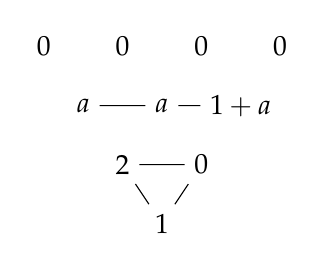
\begin{tikzpicture}
\node (41) at (-1.5,2.25) {$0$};
\node (42) at (-0.5,2.25) {$0$};
\node (43) at (0.5,2.25) {$0$};
\node (44) at (1.5,2.25) {$0$};

\node (31) at (-1,1.5) {$a$};
\node (32) at (0,1.5) {$a$};
\node (33) at (1,1.5) {$1+a$};

\node (21) at (-.5,0.75) {$2$};
\node (22) at (.5,0.75) {$0$};

\node (11) at (0,0) {$1$};

\draw (31) -- (32) -- (33) (21) -- (22) -- (11) -- (21);
\end{tikzpicture}
\qquad
\begin{tikzpicture}
\node (41) at (-1.5,2.25) {$0$};
\node (42) at (-0.5,2.25) {$a$};
\node (43) at (0.5,2.25) {$b$};
\node (44) at (1.5,2.25) {$c$};

\node (31) at (-1,1.5) {$0$};
\node (32) at (0,1.5) {$a$};
\node (33) at (1,1.5) {$b$};

\node (21) at (-.5,0.75) {$0$};
\node (22) at (.5,0.75) {$b$};

\node (11) at (0,0) {$c$};

\draw (31) -- (21) (33) -- (22);
\end{tikzpicture}
\end{Example}

\begin{Definition}
A \emph{seed} is a point $\vv \in \CC^\mu$ in normal form such that 
$\vv_{k,i} = \vv_{l,j}$ whenever $(k,i)$ and $(l,j)$ are $\vv$-related.
\end{Definition}
Notice that given $v \in \CC^\mu$ there are infinitely many seeds in
$(S_\mu \# \ZZ^\mu_0) \cdot v$. In particular there is always a seed $\vv$ 
such that $V(T(v)) \cong V(T(\vv))$, and we may always assume that our big 
module is the big module associated to a seed. 

For the rest of this section we will fix a seed $\vv$, and write $\Pi$ for 
$\Pi(v)$ and $\pi$ for the partition of $\mu$ associated to $\Pi$. We also 
write $\Desc{\pi}$ for all $z \in \ZZ^\mu_0$ such that $z_{k,i} > z_{k,j}$
whenever $i<j$ and $(k,i), (k,j)$ are $\vv$-related. In other words, $z \in
\Desc{\pi}$ if and only if $z(I)$ is a decreasing sequence for all $I \in
\Pi$. With this notation the derived tableaux basis for the module 
$V(T(\vv))$ is
\begin{align*}
\{D_\sigma(\vv + z) \mid z \in \Desc{\pi}, \sigma \in S_\pi^z\}.
\end{align*}

\paragraph
\about{Dominance relation}
\label{dominance-relation}
Let $r \in \NN$. We denote by $\Desc{r}$ the set of all descending sequences
of integers of length $r$, i.e. those $z = (z_1, z_2, \ldots, z_r) \in \ZZ^r$
with $z_1 \geq z_2 \geq \cdots \geq z_r$. Given $z, w \in \ZZ^r$ we will say
that $z$ \emph{dominates} $w$, and denote this by $z \succeq w$, if $z_i \geq 
w_i$ for all $i \in \interval{r}$ and whenever $z_i > w_i$ we have $z_1 > z_2
> \cdots > z_i$. 

For each $z \in \ZZ^r$ we denote by $S_z$ the stabilizer of $z$ in $S_r$, and
by $S^z$ the set of minimal length representatives of $S_r/S_z$, which we will
call \emph{$z$-shuffles}. 
\begin{Lemma*}
Let $z \in \ZZ^r$ and $w \in \Desc{r}$. If $z \succeq w$ then $z \in 
\Desc{r}$, and every $w$-shuffle is a $z$-shuffle.
\end{Lemma*}
\begin{proof}
The first statement is obvious from the definition. For the second, recall that
$\sigma \in S_r$ is a $z$-shuffle if and only if whenever $z_i = z_j$ and 
$i<j$ then $\sigma(i) < \sigma(j)$. Now if $z \succeq w$ then $z_i = z_j$
implies $w_i = w_j$, so every $w$-shuffle is a $z$-shuffle.
\end{proof}

\paragraph
\about{Dominance in $\Desc{\pi}$}
\label{pi-dominance-relation}
Let $z,w \in \ZZ^\mu_0$. We will say that $z$ \emph{$\vv$-dominates} $w$ and 
write $z \succeq_{\vv} w$ if $z(I) \succeq w(I)$ for each $I \in \Pi$. It 
follows from the Lemma in \ref{dominance-relation} that if $z \succeq_{\vv} w$
and $w \in \Desc{\pi}$ then $z \in \Desc{\pi}$, and $S_\pi^z \subset S_\pi^w$. 
We will usally ommit the subindex $\vv$ from $\succeq_{\vv}$.

\paragraph
\label{omega-set}
\about{The set $\Omega$}
Let $v \in \CC^\mu$ and $z \in \ZZ^\mu_0$. We set
\begin{align*}
\Omega(v)
	&= \{(k,i,j) \mid \vv_{k,i} - \vv_{k-1,j} \in \ZZ\}; \\
\Omega^+_v(z)
	&= \{(k,i,j) \in \Omega(v) \mid z_{k,i} - z_{k-1,j} 
		\in \ZZ_{\geq 0}\}.
\end{align*}
Since $\vv$ is fixed we set $\Omega = \Omega(\vv)$ and $\Omega^+(z) = 
\Omega_{\vv}^+(z)$. Given $z, z' \in \Desc{\pi}$ set $w_{k,i} = \max\{z_{k,i}, 
z'_{k,i}\}$. It follows easily from the definitions that $\Omega^+(z) \cap 
\Omega^+(z') \subset \Omega^+(w) \subset \Omega^+(z) \cup \Omega^+(z')$. 

\begin{Lemma*}
Let $z, z' \in \Desc{\pi}$ and assume $z \succeq z'$. Then there exists a 
sequence $z = z^{(0)} \succ z^{(1)} \succ \cdots z^{(r)} = z'$ such that the 
following hold for each $s \in \interval r$.
\begin{enumerate}
\item 
\label{i:delta}
There exists $(k_s, i_s) \in \Sigma$ such that $z^{(s+1)} = z^{(s)} - 
\delta^{(k_s, i_s)}$.

\item 
\label{i:interval}
The set $I_s = \{j \mid z^{(s)}_{k,j} = z^{(s)}_{k_s, i_s}\}$ is an interval 
of the form $\interval{i_s,j_s}$. 

\item 
\label{i:longest}
Let $\alpha_s$ be the cycle $(i_s i_s+1 \cdots j_s)_{(k_s)} \in S_\pi$, and
let $\omega^{(s)}$ be the unique $z^{(s)}$-shuffle in the coclass of the
longest word of $S_\pi$. Then $\omega^{(s)} = \omega^{(s-1)} \alpha(I_s)$.

\item 
\label{i:omega}
$\Omega^+(z) \cap \Omega^+(z') \subset \Omega^+(z^{(s)}) \subset \Omega^+(z) 
\cup \Omega^+(z')$.
\end{enumerate}
\end{Lemma*}
\begin{proof}
Set $\Sigma' = \{(k,i) \in \Sigma \mid z_{k,i} > z'_{k,i}\}$. If $\Sigma' =
\emptyset$ then $z = z'$ and the lemma is obvious. If $\Sigma'$ is not empty
we build a direct graph with vertex set $\Sigma'$. The directed vertices of
our graph are given by the following rules:
\begin{itemize}
\item we add an arrow $(k,i) \to (k,i+1)$ if the two entries are related;

\item we add an arrow $(k,i) \to (k-1,j)$ if $(k,i,j) \in \Omega^+(z)$;

\item we add an arrow $(k-1,j) \to (k,i)$ if $(k,i,j) \in \Omega \setminus 
\Omega^+(z)$.
\end{itemize}
The definition implies that this graph has no loops, and hence the set of 
vertices with no incoming arrows is nonempty. Among all such vertices we choose
$(k_1, i_1)$ such that $k_1$ is minimal and $i_1$ is maximal for that fixed 
$k_1$, and set $z^{(1)} = z - \delta^{(k_1, i_1)}$. We will prove that
$z^{(1)}$ satisfies all the items of the statement.

Items \ref{i:delta} and \ref{i:interval} follow immediately from the
definition. Set $\Pi^{(1)} = \Pi(z^{(1)})$ and denote by $S_\pi^{(1)}$ the
set of all $z^{(1)}$-shuffles. 
\end{proof}

\begin{bibdiv}
\begin{biblist}
\bibselect{references}
\end{biblist}
\end{bibdiv}

\end{document}